

用干净、新颖的设计编写项目文档也很重要,若把所有的工作都投入到为前沿项目编写高质量的文档中,那么必须让用户这样看到它。Doxygen拥有所有花哨的功能,但并不以紧跟最新的视觉时尚趋势而闻名。然而,这并不意味着需要付出很多努力才能改变这一点。

一个名为jothepro的开发人员创建了一个名为doxygen-awesome-css的主题,提供了一个现代的、可定制的设计,甚至有一个黑暗模式!可以在下面的截图中看到:

\begin{center}
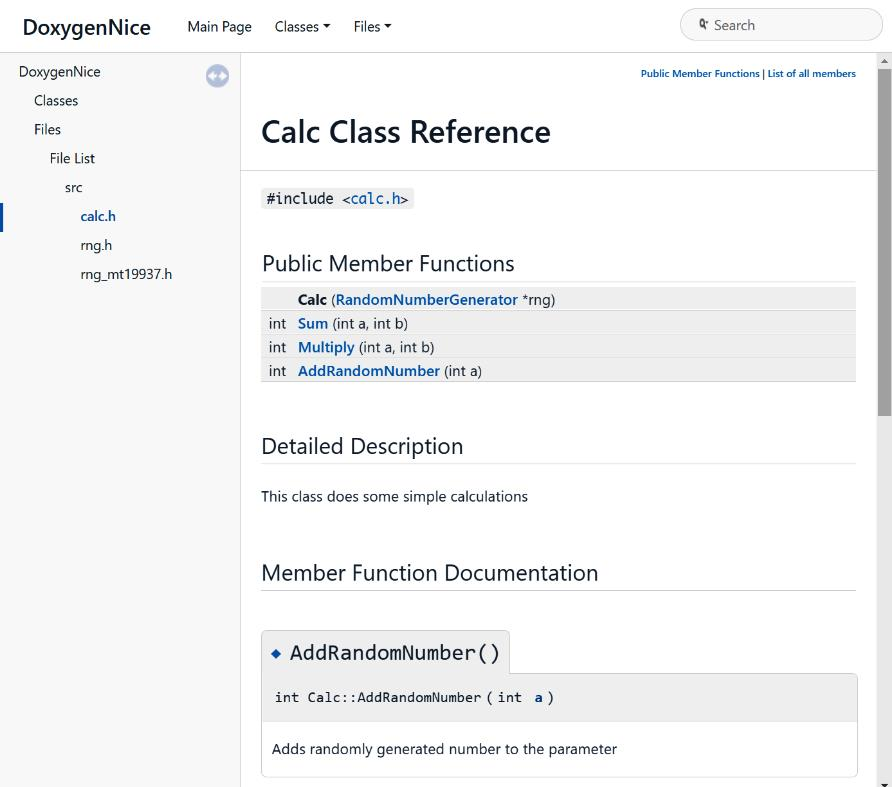
\includegraphics[width=0.8\textwidth]{content/3/chapter10/images/3.jpg}\\
图10.3  doxygen-awesome-css主题中的HTML文档
\end{center}

该主题不需要任何额外的依赖项,可以很容易地从其GitHub页面(\url{https://github.com/jothepro/doxygen-awesome-css})获取。

\begin{tcolorbox}[colback=blue!5!white,colframe=blue!75!black,title=Note]
在线教程建议使用多个应用程序串行执行来升级体验,流行的方法是使用Breathe和Exhale扩展将Doxygen的输出转换为Sphinx。这个过程看起来有点麻烦,会引入许多其他依赖项(比如Python)。我建议尽可能保持工具的简单性,很有可能不是项目中的每个开发人员都能很好地理解CMake,如此复杂的过程会给他们带来麻烦。
\end{tcolorbox}

将这个主题的自动采用,来看看如何扩展我们的Doxygen.cmake,通过添加一个新的宏来使用它:

\begin{lstlisting}[style=styleCMake]
# chapter-10/02-doxygen-nice/cmake/Doxygen.cmake (fragment)

macro(UseDoxygenAwesomeCss)
	include(FetchContent)
	FetchContent_Declare(doxygen-awesome-css
	GIT_REPOSITORY
		https://github.com/jothepro/doxygen-awesome-css.git
		GIT_TAG
		v1.6.0
	)
	FetchContent_MakeAvailable(doxygen-awesome-css)
	set(DOXYGEN_GENERATE_TREEVIEW YES)
	set(DOXYGEN_HAVE_DOT YES)
	set(DOXYGEN_DOT_IMAGE_FORMAT svg)
	set(DOXYGEN_DOT_TRANSPARENT YES)
	set(DOXYGEN_HTML_EXTRA_STYLESHEET
		${doxygen-awesome-css_SOURCE_DIR}/doxygen-awesome.css)
endmacro()
\end{lstlisting}

本书的前几章中,已经知道了所有这些命令,但为了更加清晰,来重申一下发生了什么:

\begin{itemize}
\item 
将doxy-awesome-css使用Git下载下来,并通过FetchContent模块提供给项目。

\item 
按照主题的README文件的建议,配置了Doxygen的选项。

\item 
DOXYGEN\_HTML\_EXTRA\_STYLESHEET配置主题的.css文件的路径,其将复制到输出目录。
\end{itemize}

最好在Doxygen函数中调用这个宏,就在doxygen\_add\_docs()之前:

\begin{lstlisting}[style=styleCMake]
# chapter-10/02-doxygen-nice/cmake/Doxygen.cmake

function(Doxygen input output)
	...
	UseDoxygenAwesomeCss()
	doxygen_add_docs (...)
endfunction().

macro(UseDoxygenAwesomeCss)
	...
endmacro()
\end{lstlisting}

宏中的所有变量都在调用函数的作用域中设置。

现在可以在生成的HTML文档中享受现代风格,并自信地与世界进行分享。















